% Appendix: Discrete Wavelet Transform Refresher
\chapter{Discrete Wavelet Transform Refresher}\label{app:dwt}

This appendix gives a compact mathematical refresher on the (single–level) 2-D
Discrete Wavelet Transform (DWT) used by the frequency watermark layer.

\paragraph{1-D filter bank view.} A separable orthogonal wavelet (e.g. Haar)
implements analysis via low–pass $h[n]$ and high–pass $g[n]$ filters followed by
down–sampling by 2.
For a 1-D signal $x[n]$ the approximation and detail
coefficients are
\[
  a_k = \sum_n x[n] h[2k-n],\qquad d_k = \sum_n x[n] g[2k-n].
\]
Synthesis inverts this with up–sampling and the corresponding synthesis filters.

\paragraph{2-D extension.} Applying the 1-D transform first along image rows
then columns yields four equal–sized sub-bands: LL (approximation), LH (vertical
detail), HL (horizontal detail), HH (diagonal detail). Only a single level is
required for our embedding; deeper levels increase latency and reduce spatial
localisation.

\paragraph{Energy compaction rationale.} Natural images concentrate most
variance in the LL band; embedding in selected singular values of wavelet-block
coefficients (LL or detail bands depending on robustness/imperceptibility
trade) allows small perturbations to survive moderate compression while staying
below human perceptual thresholds.

\paragraph{Why Haar?} Haar has integer coefficients (fast on edge devices) and
no boundary extension complexity; more elaborate biorthogonal wavelets (e.g.
Daubechies 9/7) marginally improve imperceptibility but raise compute cost.

\paragraph{Reference Figure.} Figure~\ref{fig:dwt_layout_ref} sketches the band
layout (single level).
The watermark selects blocks under a keyed PRNG mask.

\begin{figure}[ht]
  \centering
  % Revised 1-level DWT decomposition with intuitive feature hints
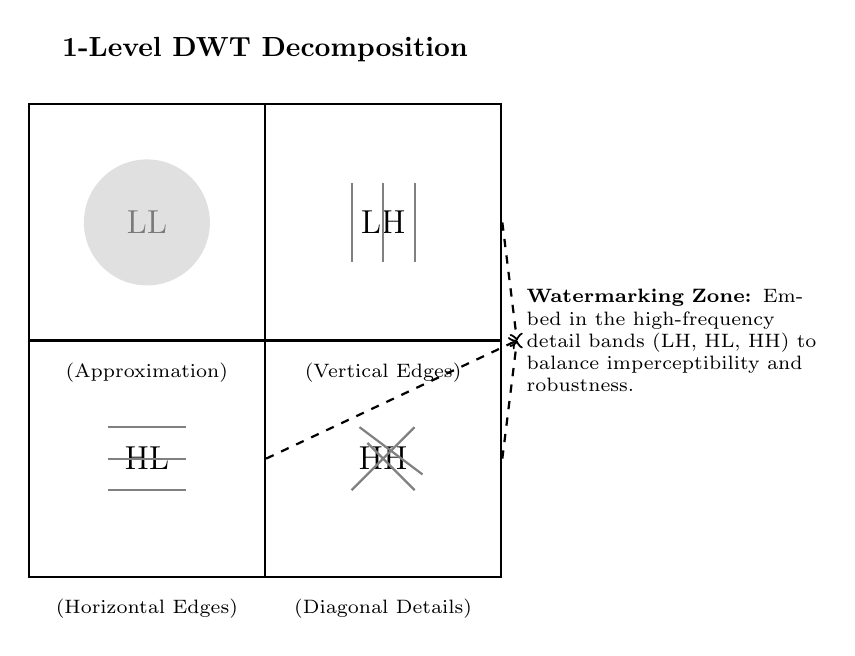
\begin{tikzpicture}[
    scale=1,
    band/.style={draw, thick, minimum width=3cm, minimum height=3cm},
    label/.style={font=\large, anchor=center},
    sublabel/.style={font=\scriptsize, anchor=north, yshift=-0.15cm},
    edgefeat/.style={gray, thick}
]
    % Title
    \node[font=\bfseries] at (3,6.7) {1-Level \gls{DWT} Decomposition};

    % Bands
    \node[band,label] at (1.5,4.5) (LL) {LL};
    \node[sublabel] at (LL.south) {(Approximation)};

    \node[band,label] at (4.5,4.5) (LH) {LH};
    \node[sublabel] at (LH.south) {(Vertical Edges)};

    \node[band,label] at (1.5,1.5) (HL) {HL};
    \node[sublabel] at (HL.south) {(Horizontal Edges)};

    \node[band,label] at (4.5,1.5) (HH) {HH};
    \node[sublabel] at (HH.south) {(Diagonal Details)};

    % Feature hints
    % LL - blurred blob
    \fill[gray!40, opacity=0.6] (1.5,4.5) circle (0.8cm);

    % LH Vertical lines
    \foreach \x in {4.1,4.5,4.9} {\draw[edgefeat] (\x,4.0)--(\x,5.0);}

    % HL Horizontal lines
    \foreach \y in {1.1,1.5,1.9} {\draw[edgefeat] (1.0,\y)--(2.0,\y);}

    % HH Diagonal snippets
    \draw[edgefeat] (4.1,1.1)--(4.9,1.9);
    \draw[edgefeat] (4.9,1.1)--(4.3,1.7);
    \draw[edgefeat] (4.2,1.9)--(5.0,1.3);

    % Annotation box
    \node[align=left, font=\scriptsize, text width=3.7cm, anchor=west] (ann) at (6.2,3.0) {\textbf{Watermarking Zone:} Embed in the high-frequency detail bands (LH, HL, HH) to balance imperceptibility and robustness.};

    % Arrows
    \draw[->, dashed, thick] (LH.east) -- (ann.west);
    \draw[->, dashed, thick] (HL.east) -- (ann.west);
    \draw[->, dashed, thick] (HH.east) -- (ann.west);
\end{tikzpicture}

  \caption{Single-level 2-D DWT band layout (LL, LH, HL, HH).}
  \label{fig:dwt_layout_ref}
\end{figure}

\paragraph[Relation to Section ref{subsec:embedding-layer}.]{Relation to Section~\ref{subsec:embedding-layer}.} The notation in
Eq.~\eqref{eq:svd_quant} assumes the block-wise \gls{svd} is applied after the \gls{dwt} on
a chosen band; this appendix formalises the transform underlying that step.
